\documentclass[11pt]{article} % scrbook otro formato
\usepackage[utf8]{inputenc}
\usepackage[spanish,es-tabla,es-nodecimaldot]{babel}

% Paquetes

\usepackage{amsmath}
\usepackage{amsthm}
\usepackage{amsfonts}
\usepackage{amssymb}
\usepackage{makeidx}
\usepackage{graphicx}
\usepackage{lmodern}
%\usepackage{kpfonts}
\usepackage{fancyhdr}
\usepackage{geometry}
\usepackage{lastpage}
\usepackage{array} % Para fjar tamaño de columnas
\RequirePackage{siunitx}
\usepackage{extramarks} % Para poder usar firstleftmarks
\usepackage[version=4]{mhchem} % Para poder usar formulas de reacciones nucleares
\usepackage{xcolor}
%\usepackage{newtxtext, newtxmath} % Cambia la fuente (pero mola)

%##############################################################################
%######### Ponemos el decimal con . ###########################################
%##############################################################################

\sisetup{output-decimal-marker={.},
	% exponentes ------------------------
	%exponent-mode=threshold,
	%exponent-thresholds=-3:2, % non usar exponentes 10^{-2,-1, 0, 1}
	% redondear -------------------------
	% round-mode=figures, % cifras sig
	% round-mode=places, % cantos decimales
	round-mode=uncertainty, % cifras sig da incerteza (necesario usar erro)
	round-precision=2,
	uncertainty-mode = separate,
	print-unity-mantissa=false,
	% unidades --------------------------
	inter-unit-product = \ensuremath{{}\cdot{}}, % separacion entre unidades
	% per-mode=power-positive-first, % so furrula con metodo interpretado puro
	inline-per-mode=single-symbol,
	display-per-mode=fraction,
}

%##############################################################################
%######### Para codigo python #################################################
%##############################################################################

\definecolor{codegreen}{rgb}{0,0.6,0}
\definecolor{codegray}{rgb}{0.5,0.5,0.5}
\definecolor{codepurple}{rgb}{0.58,0,0.82}
\definecolor{backcolour}{rgb}{0.95,0.95,0.92}

\usepackage{listings}


%\lstdefinestyle{mystyle}{	backgroundcolor=\color{backcolour},   	commentstyle=\color{codegreen},	keywordstyle=\color{magenta},	numberstyle=\tiny\color{codegray},	stringstyle=\color{codepurple},	basicstyle=\ttfamily\footnotesize,	breakatwhitespace=false,         	breaklines=true,                 	captionpos=b,                    	keepspaces=true,                 	numbers=left,                    	numbersep=5pt,                  	showspaces=false,                	showstringspaces=false,	showtabs=false,                  	tabsize=2}

%\lstset{style=mystyle}
%\usepackage{background}     % Para manejar el fondo


%##############################################################################
%######### Tipo de fuente #################################################
%##############################################################################

%\usepackage{kpfonts}

%\usepackage{helvet} 
%\renewcommand{\familydefault}{\sfdefault}.

%\usepackage{fontspec} % Paquete necesario para seleccionar fuentes
%\setmainfont{Verdana} % Cambia la fuente principal a Verdana


%##############################################################################
%######### Geometría #################################################
%##############################################################################

\geometry{a4paper, total={152mm,237mm}, left=31mm, top=30mm}



%##############################################################################
%######### Formatos capítulo #################################################
%##############################################################################

%\usepackage[lmodern]{quotchap}
%\usepackage[Bjornstrup]{fncychap}

% Para el Bjornstrup
%\ChNumVar{\fontsize{76}{80}\usefont{OT1}{pzc}{m}{n}\selectfont}
%\ChTitleVar{\raggedright\Huge\sffamily\bfseries}


%##############################################################################
%######### Hiperreferenias #################################################
%##############################################################################


\usepackage[colorlinks=true,allcolors=blue]{hyperref} % Crea las


%##############################################################################
%######### Formato de pagina #################################################
%##############################################################################

%\renewcommand{\chaptermark}[1]{\markboth{\chaptername\ \thechapter.\ #1}{}}
\renewcommand{\sectionmark}[1]{\markright{\thesection.\ #1}}

\setlength{\headsep}{27pt} % Distancia entre la cabezera y el texto
\setlength{\footskip}{30pt} % Distancia entre el pie de pagina y el texto
\pagestyle{fancy}
\fancyhf{}
\fancyhead[LE]{\rightmark} % L,R,C-> left, right, center [LE,RO]
\fancyhead[RO]{\rightmark} % E,O -> even (par), odd (impar)
\fancyhead[LO,RE]{Daniel Vázquez Lago}
\fancyfoot[CE,CO]{\thepage}
\renewcommand{\headrulewidth}{1pt} % Cambiamos el grosor de la linea de arriba
\renewcommand{\footrulewidth}{0pt}



%##############################################################################
%#########  Modificar caption #################################################
%##############################################################################

\usepackage[font=small, justification=centering]{caption}  % Configura las captions



%##############################################################################
%######### Comandos propios #################################################
%##############################################################################

\newcommand{\parentesis}[1]{\left( #1  \right)} 
\newcommand{\parciales}[2]{\frac{\partial #1}{\partial #2}}
\newcommand{\pparciales}[2]{\parentesis{\parciales{#1}{#2}}}
\newcommand{\ccorchetes}[1]{\left[ #1  \right]}
\newcommand{\D}{\mathrm{d}}
\newcommand{\derivadas}[2]{\frac{\D #1}{\D #2}}

\newcommand{\tquad}{\quad \quad \quad}
\newcommand{\vnabla}{\vec{\nabla}}

\newcommand{\Ocal}{\mathcal{O}}
\newcommand{\Ncal}{\mathcal{N}}
\newcommand{\Hcal}{\mathcal{H}}

\newcommand{\logd}{\log_{10}}

\newcommand{\eV}{\text{eV}}
\newcommand{\cm}{\text{cm}}
\newcommand{\cmm}{\text{cm}^{-1}}
\newcommand{\fm}{\text{fm}}
\newcommand{\He}{\text{He}}
\newcommand{\p}{\text{p}}
\newcommand{\e}{\text{e}}
\newcommand{\cte}{\text{cte}}


% Comandos vectoriales

\newcommand{\an}{\mathbf{a}}
\newcommand{\bn}{\mathbf{b}}
\newcommand{\dn}{\mathbf{d}}
\newcommand{\jn}{\mathbf{j}}
\newcommand{\lnn}{\boldsymbol{\ell}}
\newcommand{\lnnn}{\boldsymbol{l}}
\newcommand{\kn}{\mathbf{k}}
\newcommand{\pn}{\mathbf{p}}
\newcommand{\qn}{\mathbf{q}}
\newcommand{\rn}{\mathbf{r}}
\newcommand{\sn}{\mathbf{s}}
\newcommand{\un}{\mathbf{u}}
\newcommand{\vn}{\mathbf{v}}
\newcommand{\xn}{\mathbf{x}}
\newcommand{\yn}{\mathbf{y}}
\newcommand{\qndot}{\dot{\qn}}

\newcommand{\unovec}{\vec{\mathbf{1}}}

\newcommand{\alphan}{\boldsymbol{\alpha}}
\newcommand{\sigman}{\boldsymbol{\sigma}}
\newcommand{\pin}{\boldsymbol{\pi}}


\newcommand{\An}{\mathbf{A}}
\newcommand{\Bn}{\mathbf{B}}
\newcommand{\En}{\mathbf{E}}
\newcommand{\Gn}{\mathbf{G}}
\newcommand{\Jn}{\mathbf{J}}
\newcommand{\Kn}{\mathbf{K}}
\newcommand{\Ln}{\mathbf{L}}
\newcommand{\Rn}{\mathbf{R}}
\newcommand{\Sn}{\mathbf{S}}
\newcommand{\Tn}{\mathbf{T}}
\newcommand{\In}{\mathbf{I}}

\newcommand{\hnn}{\hat{\mathbf{n}}}
\newcommand{\hnr}{\hat{\mathbf{r}}}
\newcommand{\hnz}{\hat{\mathbf{z}}}
\newcommand{\hnx}{\hat{\mathbf{x}}}
\newcommand{\hny}{\hat{\mathbf{y}}}
\newcommand{\hnu}{\hat{\mathbf{u}}}
\newcommand{\hnR}{\hat{\mathbf{R}}}
\newcommand{\hnv}{\hat{\mathbf{v}}}
\newcommand{\hnk}{\hat{\mathbf{k}}}
\newcommand{\hni}{\hat{\mathbf{i}}}
\newcommand{\hnj}{\hat{\mathbf{j}}}
\renewcommand{\hnk}{\hat{\mathbf{k}}}





%##############################################################################
%######### Teoremas/definiciones #################################################
%##############################################################################

%\theoremstyle{definition}
%\newtheorem{definition}{Definición}[chapter]
%\theoremstyle{theorem}
%\newtheorem{theorem}{Teorema}[chapter]




%##############################################################################
%######### Referncia para euccaiones y figuras ################################
%##############################################################################

%\numberwithin{equation}{section}
%\numberwithin{figure}{section}




%##############################################################################
%######### Documento #################################################
%##############################################################################


\author{Daniel Vazquez Lago}
\title{Simulación en física de materiales}


\begin{document}	
	
\maketitle
\newpage
\tableofcontents
\section{Objetivos}
	
El objetivo de este primer optativo es estudiar si realmente, tras los $\num{5e5}$ pasos, hemos llegado a una configuración de equilibrio. Para esto presentaremos 3 diferentes condiciones que un sistema aislado en equilibrio debería satisfacer (\cite{Haile}):

\begin{itemize}
 	\item La energía $E$ total debe mantenerse constante en el tiempo, a poder ser $E=-575$.
 	\item Los valores medios de las velocidades (cada una de las componentes) deben seguir distribuciones de Maxwell.
 	\item La función $H$ de Boltzmann debe tender a un valor constante. 	
\end{itemize}
Existen mas condiciones que no trataremos aquí, no por otra cosa que la falta de información. Sin embargo, ninguna de estas (individualmente y colectivamente) nos garanticen de manera completamente inequívoca que estamos en el equilibrio.
	
\section{Organización}
	
\section{Equilibración}

En esta sección vamos a estudiar desde una perspectiva teórica cuales son las condiciones de equilibrio, para luego ver cuales son los resultados según cada una de estas condiciones. En esta sección usaremos sobretodo el contenido que aparece en las páginas 206-209 del Haile \cite{Haile}. 

\subsection{Energía total constante}

\subsubsection{Teoría}

Esta condición nos asegura que el si $E$ es constante en el tiempo, de tal manera que las fluctuaciones de la energía cinética y energía potencial deben ser contrarias, esto es, cuando una de ellas aumente la otra debe disminuir y viceversa. 

Esta es el estudio más sencillo de todos, y no se uso un archivo de fortran para ello, si no de python. La razón por la cual se hace así

\subsubsection{Resultados}

	
\subsection{Distribución de Velocidades}
	
\subsubsection{Teoría}

En este apartado vamos a seguir el desarrollo hecho en el \cite{Haile} (pag. 65-66, pag. 120). Para una distribución de velocidades en el equilibrio (colectividad NVT) verifica que, para cada una de las componentes $i$ de las velocidades ($v_x,v_y,v_z$), dado que son independientes: 

\begin{equation}
	f(v_i) = \sqrt{\frac{m}{2\pi k T}} \exp \parentesis{- \frac{mv_i}{2kT}}
\end{equation}
Aunque la distribución de Maxwell halla sido derivada en el formalismo de la colectividad canónica (NVT, PVT...), la distribuciones de cualquier sistema en el equilibrio debería ser de este tipo, ya que en el límite termodinámico las propiedades en las diferentes colectividades se vuelven equivalentes. \\

Una de las consecuencias de la distribución de velocidades es la equipartición de la energía, por lo las componentes cartesianas de la velocidades moleculares deberían tener un valor medio igual al de la temperatura del sistema:

\begin{eqnarray}
	\frac{1}{N} \left\langle \sum_i v_{ix}^2 \right\rangle = 
	\frac{1}{N} \left\langle \sum_i v_{ix}^2 \right\rangle = 
	\frac{1}{N} \left\langle \sum_i v_{ix}^2 \right\rangle = T
\end{eqnarray}
\subsubsection{Resultados}
\begin{figure}[h!] \centering
	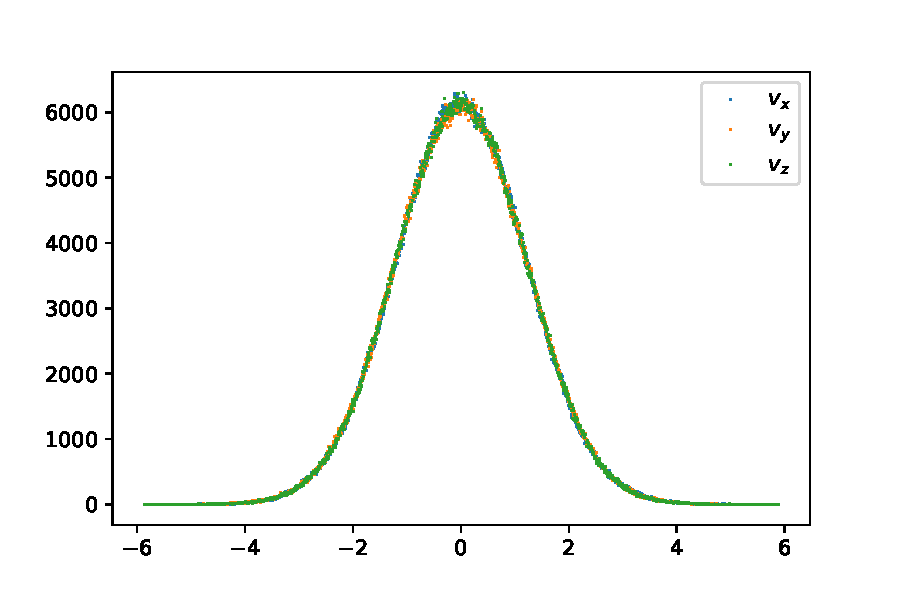
\includegraphics[width=1.0\textwidth]{../../Graficas/Velocidades_histo.pdf}
	\caption{valores de las funciones de Maxwell $H_x$, $H_y$ y $H_z$ con el tiempo.}
	\label{Fig:03}
\end{figure}	

	
\subsection{Distribución $H$-Boltzmann} 	
\subsubsection{Teoría}

En este apartado vamos a seguir el desarrollo hecho en el \cite{Haile} (pag. 66-67, pag. 120-121). Definimos la función $H$ de Boltzmann (función $H$) en un instante $t$ como:

\begin{eqnarray}
	H_i(t) = \int_{-\infty}^{\infty} f(v_i) \ln (f(v_i)) \D v_i \tquad i = x,y,z
\end{eqnarray} 
de tal modo que podemos definir la $H$ de Boltzmann como
\begin{eqnarray}
	H=\frac{1}{3} \parentesis{H_x+H_y+H_z}
\end{eqnarray}

El \textbf{teorema H de Boltzmann} asegura que una distribución llega al equilibrio cuando se alcanza un mínimo en la función $H$ de Boltzmann, dada por la anterior ecuación. Sin embargo nosotros no podemos implementar integrales, si no sumatorios (las integrales tienen un carácter infinitesimal que no podemos alcanzar con el ordenador), por lo que nosotros tendremos que implementar:

\begin{equation}
	H_i (t) = \sum_{\Delta v_i} f(v_i) \ln (f(v_i)) \Delta v_i  \tquad i=x,y,z
\end{equation}
donde

\begin{equation}
	f(v_x) \Delta v_x = \frac{1}{N} \sum_i^N \delta (v_x-v_{xi}) \Delta v_x
\end{equation}
e igual para $v_y$ e $v_z$. 

\subsubsection{Resultados}
	
	
	\begin{figure}[h!] \centering
		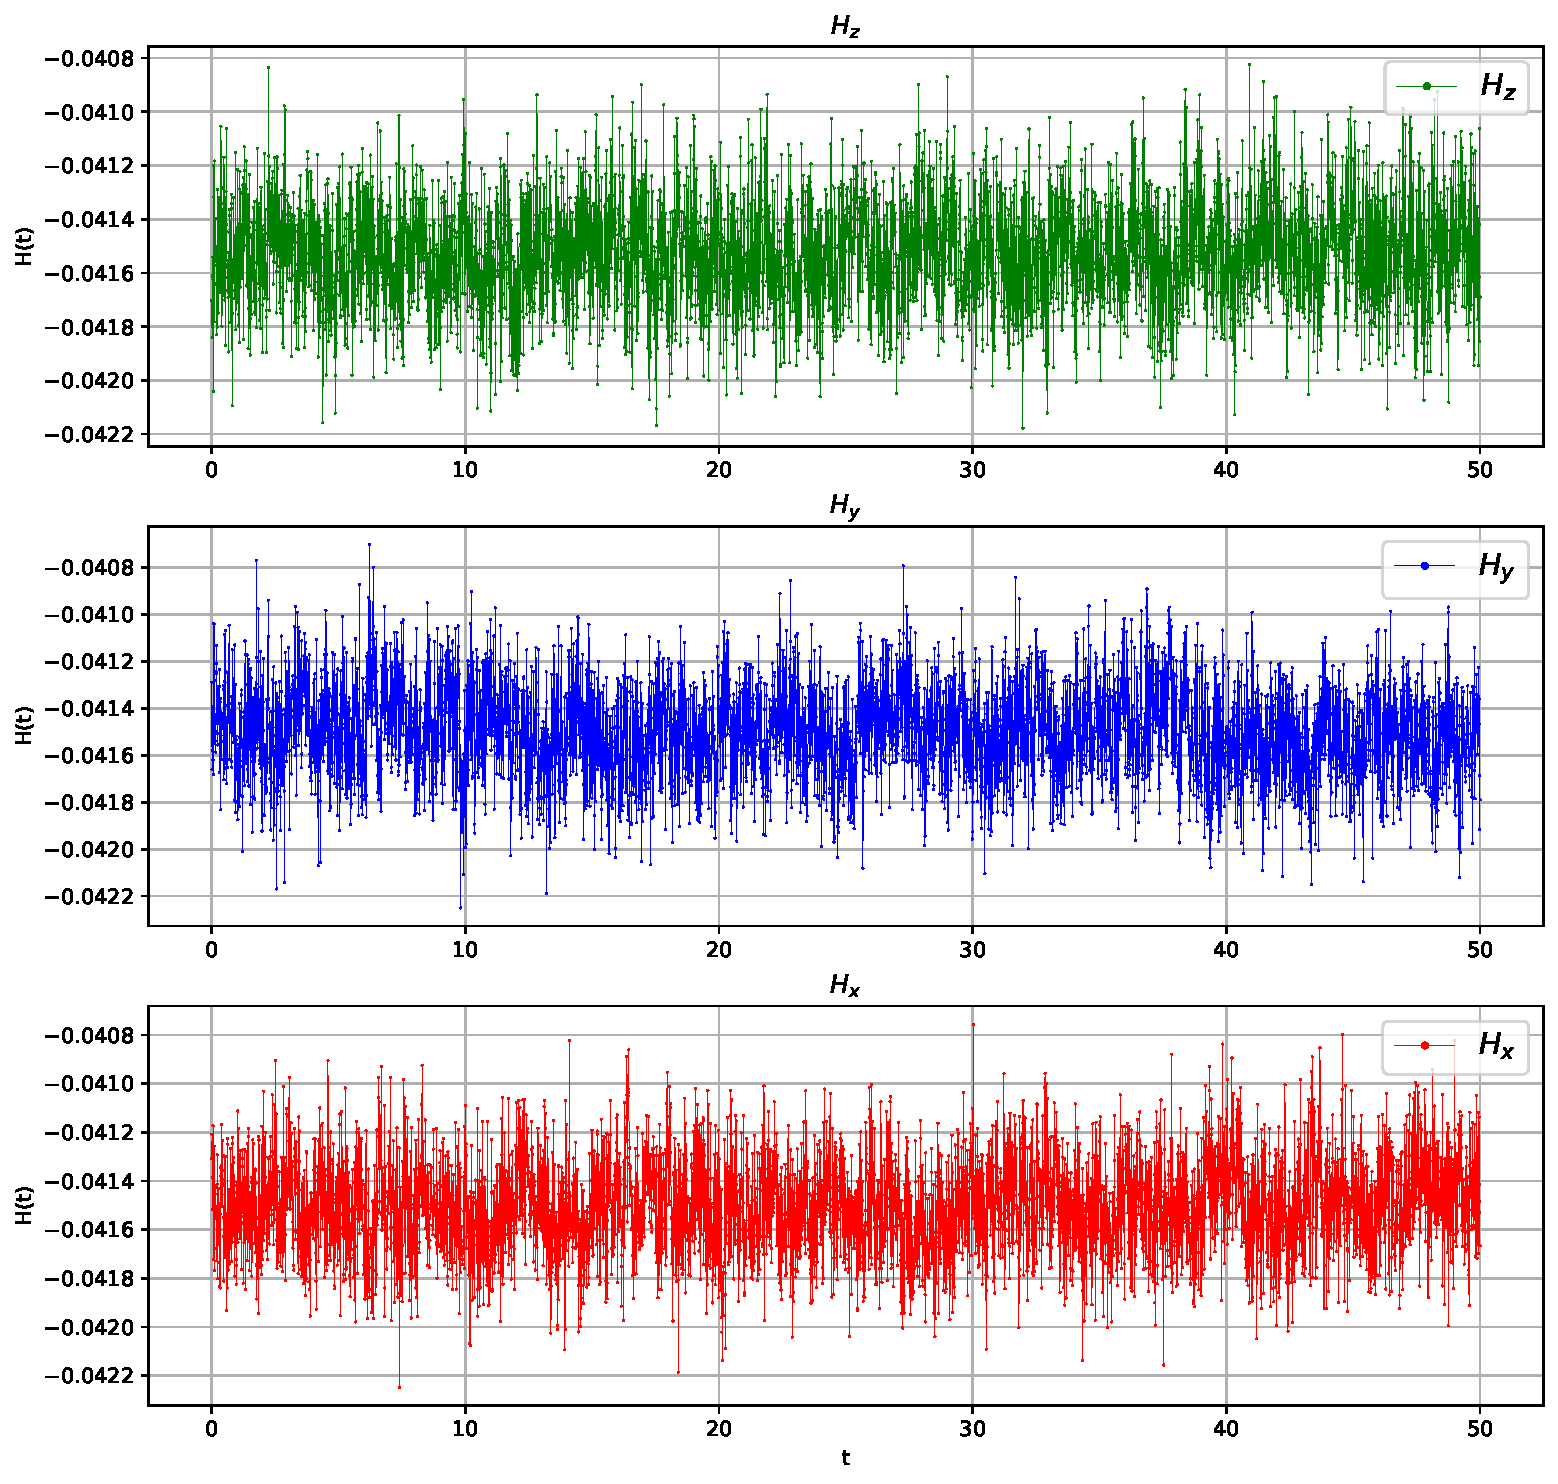
\includegraphics[width=1.0\textwidth]{../../Graficas/H_Boltzmann_xyz.pdf}
		\caption{valores de las funciones de Maxwell $H_x$, $H_y$ y $H_z$ con el tiempo.}
		\label{Fig:05}
	\end{figure}
	
	\begin{figure}[h!] \centering
		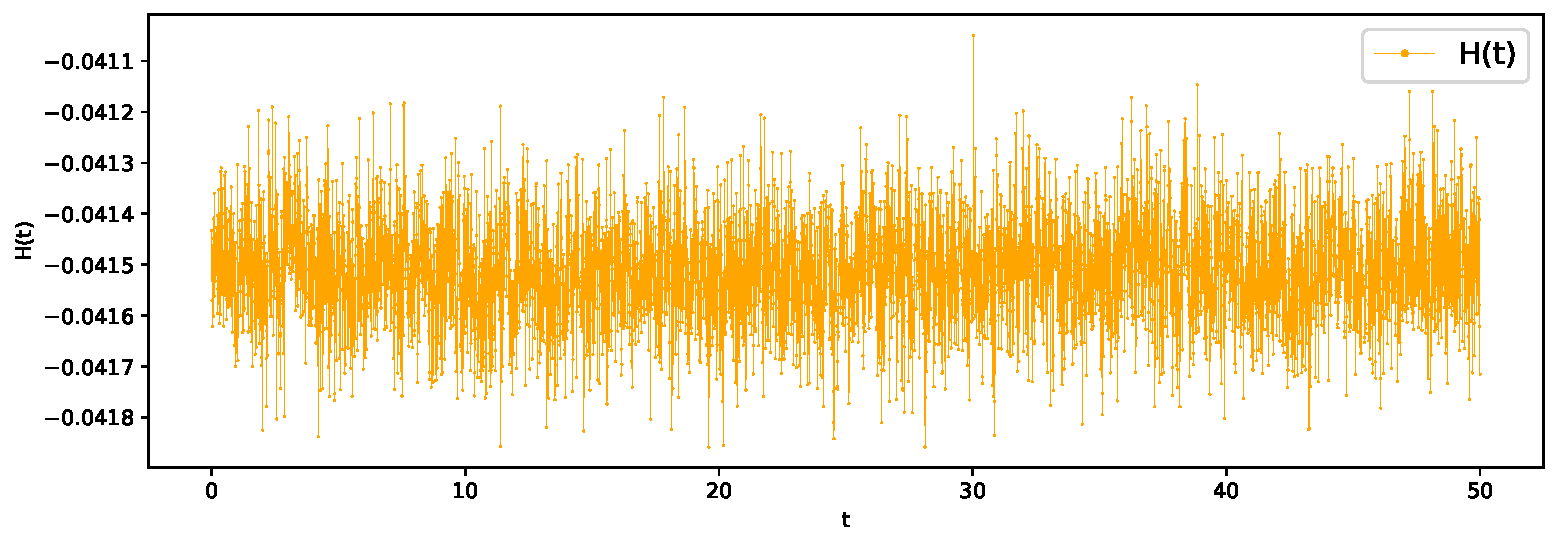
\includegraphics[width=1.0\textwidth]{../../Graficas/H_Boltzmann.pdf}
		\caption{Valor de la función de Maxwell $H(t)$ con el tiempo .}
		\label{Fig:04}
	\end{figure}	
	
	
\section{Conclusiones}
	
	
\bibliography{Bibliografia.bib}
\bibliographystyle{unsrt}
	
	
\end{document}	
